\documentclass[11pt,a4paper]{article}
\usepackage[utf8]{inputenc}
\usepackage[T1]{fontenc}
\usepackage[romanian]{babel}
\usepackage[margin=2cm]{geometry}
\usepackage{array}
\usepackage{tabularx}
\usepackage{enumitem}
\usepackage{graphicx}
\usepackage{setspace}
\usepackage{xcolor}
\usepackage{hyperref}
\usepackage{amssymb}
\setlength{\parindent}{0pt}
\newcommand{\fillline}[1][6cm]{\underline{\hspace{#1}}}
\newcommand{\fillbox}[1][0.4cm]{\framebox[#1]{\rule{0pt}{#1}}}
\newcommand{\checkboxempty}{$\square$}

\begin{document}

\noindent
\begin{minipage}[t]{0.40\textwidth}
\vspace{0pt}
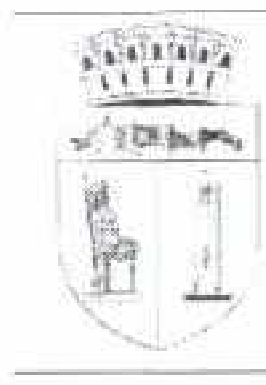
\includegraphics[height=1.5cm]{../assets/stema-cluj.png}%
\hspace{0.2cm}%
\raisebox{0.5cm}{\parbox[t]{3.5cm}{\textbf{PRIMĂRIA}\\\textbf{CLUJ-NAPOCA}}}
\end{minipage}%
\begin{minipage}[t]{0.30\textwidth}
\centering
\vspace{0.4cm}

\includegraphics[width=3.5cm,height=0.9cm]{../assets/barcode-304001.png}
\end{minipage}%
\begin{minipage}[t]{0.30\textwidth}
\raggedleft
\vspace{0.6cm}
Nr. \fillline[3cm] / \fillline[1cm]
\end{minipage}

\vspace{0.3cm}
\hrule
\vspace{0.6cm}

\textbf{Către,}

\vspace{0.2cm}

\hspace{1cm}\textbf{Primăria Municipiului Cluj-Napoca}

\vspace{0.7cm}

\hspace{1cm}Subsemnatul (a) \fillline[10cm], având CNP \fillline[5cm], domiciliat (ă) în localitatea \fillline[5cm], strada (comuna) \fillline[6cm], nr (sat) \fillline[3cm], bl. \fillline[1.5cm], sc. \fillline[1.5cm], et. \fillline[1.5cm], ap. \fillline[1.5cm], judeţul (sectorul) \fillline[4cm], posesor al actului de identitate seria \fillline[1.5cm], nr. \fillline[3cm], eliberat la data de \fillline[3cm] de \fillline[5cm], prin prezenta doresc să semnalez prezenţa speciei alergene ambrozia (\textit{Ambrosia artemisiifolia}) în zona (descriere cât mai detaliată, strada, nr., longitudine, latitudine) \fillline[6cm]

\vspace{0.2cm}

\hrulefill

\vspace{0.2cm}

\hrulefill

\vspace{0.2cm}

\hrulefill

\vspace{0.5cm}

Numărul aproximativ al tufelor de ambrozie: \fillline[8cm]

\vspace{0.3cm}

Mărimea zonei afectate (mp): \fillline[8cm]

\vspace{0.4cm}

Tipul zonei afectate:
\begin{itemize}[leftmargin=2cm,label=\checkboxempty]
\item îngrădit
\item neîngrădit
\end{itemize}

\vspace{0.2cm}

Categoria de folosinţă a terenului:
\begin{itemize}[leftmargin=2cm,label=\checkboxempty]
\item arabil
\item păşune
\item fâneaţă
\item livadă
\item curţi-construcţii
\item grădină
\item teren abandonat/neîntreţinut
\item alte categorii de folosinţă
\end{itemize}

\vfill
\hrule
\vspace{0.3cm}

\begin{minipage}[t]{0.65\textwidth}
www.primariaclujnapoca.ro\\
telefon: 0264/596.030\\
Cluj-Napoca, str. Moţilor, nr. 3
\end{minipage}%
\begin{minipage}[t]{0.35\textwidth}
\raggedleft

\includegraphics[width=3cm,height=0.7cm]{../assets/barcode-304001.png}
\end{minipage}

\vspace{0.3cm}
\hrule
\vspace{0.2cm}

{\footnotesize
\textbf{Timp estimativ de completare: 10 minute}

\vspace{0.2cm}

Datele personale care vă sunt solicitate prin prezenta cerere vor fi prelucrate numai în vederea procesării și soluționării solicitării dumneavoastră. Primăria municipiului Cluj-Napoca garantează securitatea procesării datelor și arhivarea acestora în conformitate cu prevederile legale în vigoare.
}

\newpage

\noindent
\begin{minipage}[t]{0.40\textwidth}
\vspace{0pt}
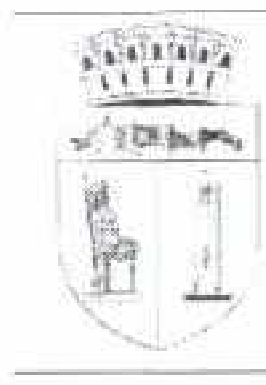
\includegraphics[height=1.5cm]{../assets/stema-cluj.png}%
\hspace{0.2cm}%
\raisebox{0.5cm}{\parbox[t]{3.5cm}{\textbf{PRIMĂRIA}\\\textbf{CLUJ-NAPOCA}}}
\end{minipage}%
\begin{minipage}[t]{0.30\textwidth}
\centering
\vspace{0.4cm}

\includegraphics[width=3.5cm,height=0.9cm]{../assets/barcode-304001.png}
\end{minipage}%
\begin{minipage}[t]{0.30\textwidth}
\raggedleft
\vspace{0.6cm}
Nr. \fillline[3cm] / \fillline[1cm]
\end{minipage}

\vspace{0.3cm}
\hrule
\vspace{0.6cm}

Proprietarul (în cazul în care se cunoaşte): \fillline[10cm]

\vspace{0.3cm}

Alte informaţii utile: \fillline[12cm]

\vspace{0.2cm}

\hrulefill

\vspace{0.6cm}

\hspace{1cm}În vederea identificării corecte a terenului vă rugăm să ataşaţi fotografii reprezentative, din care se poate recunoaşte atât specia ambrozia, cât şi zona în care s-a identificat prezenţa acesteia.

\vspace{0.6cm}

\checkboxempty\ Prin prezenta solicit comunicarea răspunsului pe următoarea adresă de e-mail:

\vspace{0.2cm}

\fillline[14cm]

\vspace{0.4cm}

\checkboxempty\ Mă oblig să comunic instituției orice modificare intervine în legătură cu această adresă de e-mail

\checkboxempty\ Îmi exprim consimțământul ca Primăria Municipiului Cluj-Napoca să comunice orice informații, date personale, clarificări și completări pe adresa de e-mail indicată mai sus

\checkboxempty\ Am luat la cunoștință faptul că în cazul nefuncționării serverului de e-mail comunicat sau în cazul adresei greșite de e-mail, Municipiul Cluj-Napoca nu poate fi tras la răspundere pentru acest lucru

\vspace{0.8cm}

Data: \fillline[4cm] \hfill Semnătura: \fillline[4cm]

\vspace{0.4cm}

Număr telefon: \fillline[5cm]

\vspace{0.3cm}

Email \fillline[7cm]

\vfill
\hrule
\vspace{0.3cm}

\begin{minipage}[t]{0.65\textwidth}
www.primariaclujnapoca.ro\\
telefon: 0264/596.030\\
Cluj-Napoca, str. Moţilor, nr. 3
\end{minipage}%
\begin{minipage}[t]{0.35\textwidth}
\raggedleft

\includegraphics[width=3cm,height=0.7cm]{../assets/barcode-304001.png}
\end{minipage}

\vspace{0.3cm}
\hrule
\vspace{0.2cm}

{\footnotesize
\textbf{Timp estimativ de completare: 10 minute}

\vspace{0.2cm}

Datele personale care vă sunt solicitate prin prezenta cerere vor fi prelucrate numai în vederea procesării și soluționării solicitării dumneavoastră.
}

\end{document}
